\section{Genetische Algorithmen}

% Was ist n Genetischer Algorithmus
Genetische Algorithmen nehmen Inspiration von der Evolutionstheorie von Charles Darwin
Dass angepasstere Individuen erfolgreicher darin sind ihre Genetischen Informationen zu verbreiten

Ein Genetischer Algorithmus arbeitet nicht mit den möglichen Lösungen selbst
sonder mit Chromosom Representationen der Lösungen. [GAs]
Ein Chromosom ist also ein Vektor Representation einer Lösung des Problems
Die einzelnen Werte eines Chromosoms nennt man Gene und eine Menge an Genen 
bilden eine Population. [Siehe Grafik 01]

% DO: Grafik Population, Gen, Individual
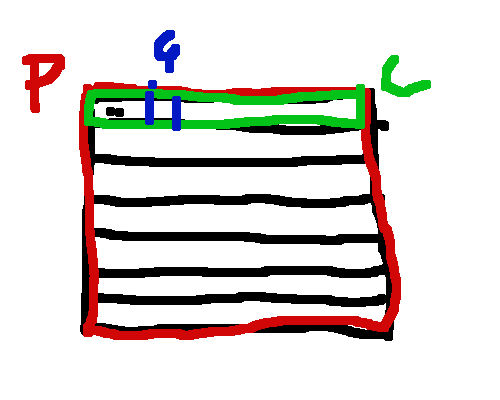
\includegraphics[scale=1.0]{images/Population_Chromosom_Gen.png}


% Key Components
Jeder Genetische Algorithmus implementiert eine 
representations Operator 
Fitness Operator
und Genetische Operatoren [missing quote]
Selection Operator
Mutation Operator
Crossover Funktion


Der Representationsoperator übersetzt eine Lösung aus dem Search space 
in ein Chromosom. 


Die Fitness Funktion weist jedem Individuum einen Wert zu anhand welchem man die 
Individuen vergleichen kann


Der Selection Operator wählt Chromosomepaare aus. Dies kann 
zufällig geschehen, meist wird der selection Operator jedoch anhand der Fitness oder Ränge ausgewählt

Der Crossover Operator erhält eine Menge an Chromosomen und rekombiniert diese
zu Kindern.
Typischerweise werden je zwei Eltern zu einem Kind rekombiniert.


Der Mutationsoperator verändert ein Chromosom zufällig

% Ablauf von genetischem Algorithmus



% Hyper Parameter des Genetischen Algorithmus
% Und worauf man bei der Belegung achten sollte
Population Size
Wählt man diese Zu gering kann es zu einer verfrühten Konvergenz und somit auch einer schlechten Lösung kommen
Gleichzeitig ist die Population size ein Maßgebender Faktor in der Rechenzeit und eine zu große Population könnte 
Rechenzeit verschwenden [GAs]




Im folgenden werde ich bekannte implementationen der genetischen Operatoren eingehen und beschreiben worauf man bei der implementation achten muss

\subsection*{Mutationsoperatoren}
Random Uniform Mutation:
Random Unifor mutation 


